% !TEX TS-program = pdflatex
\documentclass[11pt, oneside]{article}   	% use "amsart" instead of "article" for AMSLaTeX format
\usepackage{hl_short}
\usepackage{geometry}                		% See geom\dagetry.pdf to learn the layout options. There are lots.
\geometry{a4paper}                   		% ... or a4paper or a5paper or ... 
%\geometry{landscape}                		% Activate for for rotated page geometry
%\usepackage[parfill]{parskip}    		% Activate to begin paragraphs with an empty line rather than an indent
\usepackage{graphicx}				% Use pdf, png, jpg, or eps§ with pdflatex; use eps in DVI mode
\usepackage{array}							% TeX will automatically convert eps --> pdf in pdflatex		
\usepackage{amsmath,amssymb}
\usepackage{cite}
\usepackage[draft]{fixme}
\usepackage{pdfpages}
\usepackage{tabularx}
\usepackage{fancyheadings}
\usepackage{lastpage}
\usepackage{tikz}
\usetikzlibrary{trees}
\usetikzlibrary{shadows}
\usetikzlibrary{backgrounds}
\usetikzlibrary{shapes,arrows,automata}
\usetikzlibrary{positioning,intersections,fit}

\tikzset{
  shape example/.style={
    color=black!30,
    draw,
    fill=yellow!30,
    line width=.3cm,
    inner xsep=1.7cm,
    inner ysep=0.5cm}
}

%\usetikzlibrary{positioning,shapes,arrows}
\usepackage{float}
\usepackage{hyperref}
\usepackage{url}


\newcommand{\bX}{\mathbf{X}}
\newcommand{\bx}{\mathbf{x}}
\newcommand{\bU}{\mathbf{U}}
\newcommand{\bu}{\mathbf{u}}
\newcommand{\bE}{\mathbf{E}}
\newcommand{\be}{\mathbf{e}}
\renewcommand{\bmu}{\boldsymbol{\mu}}
\newcommand{\bSigma}{\boldsymbol{\Sigma}}
\renewcommand{\trans}{^{\mathsf{T}}}

\renewcommand{\comment}[1]{\begin{center}\textbf{[[  #1 ]]}\end{center}}
\parskip 6pt % 1pt = 0.351 mm
\parindent 0pt

\pagestyle{fancy}
\lhead{\tiny FP7-ICT 619209 / AMIDST}
\chead{\tiny Page {\thepage} of \pageref{LastPage} \\}
\rhead{\tiny Public}
\renewcommand{\footrulewidth}{0.4pt}
\cfoot{}

\newcommand{\drop}[1]{}


\usepackage{tikz}
\usetikzlibrary{bayesnet}


\begin{document}



% Table of contents
\tableofcontents

\newpage

% Document History

\section*{Document history}

\begin{table}[htbp]
  \centering
  \begin{tabularx}{\linewidth}{|p{17mm}|p{17mm}|X|X|}\hline
    {\bf Version} & {\bf Date} & {\bf Author (Unit)} & {\bf Description} \\ \hline \hline
    v0.3 & 21/11 2014 & Helge Langseth, Thomas D. Nielsen,   Antonio Salmer\'on & First draft   \\ \hline
\hline
  \end{tabularx}
\end{table}

\newpage


% Document History

\section{Executive summary}

The aim of this document is to describe the progress of the software development related to learning in the AMIDST project at the end of the first year. 



 
\newpage

% 1. Welcome. This is a BN, and we want to learn it.
% !TEX root = D41-report.tex
\section{Introduction}

\comment{This is just the first  page from D3.1, then quickly terminated after learning is introduced. Just to say what a BN is.}


Probabilistic graphical models provide a well-founded and principled approach for performing inference 
in complex domains endowed with uncertainty. A probabilistic graphical model is a framework consisting 
of two parts: a qualitative component in the form of a graphical model encoding conditional independence 
assertions about the domain being modelled as well as a quantitative component consisting of a collection of local 
probability distributions adhering to the independence properties specified in the graphical model. Collectively, the 
two components provide a compact representation of the joint probability distribution over the domain being modelled. 

Bayesian networks (BNs) \cite{Pearl88} are a particular type of
probabilistic graphical model that has enjoyed widespread attention in
the last two decades. Figure~\ref{fig:sampleBN} shows a BN representing
the joint distribution of variables $X_1,\ldots,X_5$. Attached to each node, there is a conditional probability
distribution given its parents in the network, so that the joint distribution factorises as

\[
p(X_1,\ldots,X_5) = p(X_1) p(X_2|X_1) p(X_3|X_1) p(X_4|X_2,X_3) p(X_5|X_3).
\]

In general, for a BN with $n$ variables $\bX=\{X_1,\ldots,X_n\}$, the joint distribution factorises as

\begin{equation}
\label{equ:factorisation}
p(\bX) = \prod_{i=1}^n p(X_i|\pa{X_i}) ,
\end{equation}
where $\pa{X_i}$ denotes the set of parents of $X_i$ in the network. 


\newcommand{\simpleModel}{    
      \node[obs] (X1) {$X_1$};
      \node[obs] (X2) [below left of=X1, xshift=-1.2cm, yshift=-1.2cm] {$X_2$};
      \node[obs] (X3) [below right of=X1, xshift=+1.2cm, yshift=-1.2cm] {$X_3$};
      \node[obs] (X4) [below right of=X2, xshift=+1.2cm, yshift=-1.2cm] {$X_4$};
      \node[obs] (X5) [below right of=X3, xshift=+1.2cm, yshift=-1.2cm] {$X_5$};
      \edge{X1}{X2};
      \edge{X1}{X3};
      \edge{X2,X3}{X4};
      \edge{X3}{X5};
    }
    
\begin{figure}[htb]
  \begin{center}
   \scalebox{1}{
    \begin{tikzpicture}

    \simpleModel
    \end{tikzpicture}
    }
  \end{center}
  \caption{A Bayesian network with five variables.}
  \label{fig:sampleBN}
\end{figure}


We will use lowercase letters to refer to
values or configurations of values, so that $x$ denotes a value of $X$ and $\bx$ is a configuration of the
variables in $\bX$. 
Given a set of observed variables $\bX_E\subset \bX$ and a set of variables of interest $\bX_I\subset \bX \setminus \bX_E$,
\emph{probabilistic inference} is the calculation  of the posterior distribution
$p(x_i|\bx_E)$ for each $i\in I$. 
A thorough introduction to the state of the art for inference in Bayesian networks was given in \cite{D3.1}. 

In this document we assume that inference techniques for a given Bayesian network is available, and will consider how to define a Bayesian network model that fits a data set as well as possible.
This process is known as \textit{learning} in the Bayesian network community.






% 2. The idea of using a Bayesian approach, where the parameters we will learn are explicitly represented and inference
%  (VB etc) in fact superimposes parameter-learning.
% !TEX root = D41-report.tex


\section{Learning Bayesian networks} \label{sec:learningAsInference}

%\comment{Say that we recommend the use of a fully Bayesian approach. Approximate inference techniques (VB / EP, importance sampling, etc) can be optimized for the model class. Maximum likelihood based approaches do not go well hand in hand with approximate inference techniques...}

Consider again the factorization of the full joint distribution $p(\bx)$ in \equref{factorisation}. With this factorization we can efficiently represent the joint probability distribution $p(\bx)$, but it requires that $\pa{X_i}$, i.e., the \textit{parent set} of  $X_i$, is known for each $i=1\ld n$. 
The parents of $X_i$ are exactly the nodes which have an outgoing edge pointing to $X_i$ (e.g., $\pa{X_4}=\{X_2,X_3\}$ for the model in \figref{sampleBN}). 
Algorithms for learning the parent sets, also denoted \textit{structural learning} algorithms, follow one of two approaches: $i)$ search and score  methods, see e.g. \cite{CooperHerskovitz92} and $ii)$ constraint-based techniques \cite{SGS}. Both will be considered in Task 4.1 of the project, and the progress towards the implementation of structural learning in AMIDST is summarized in \secref{parallel}.

As soon as the parent sets in  \equref{factorisation} are determined, the specific conditional distributions $p(X_i\given\pa{X_i})$ can also be learned from data. The approach taken in the AMIDST project is that the conditional distribution $p(X_i\given\pa{X_i})$ is assumed to belong to a specific distributional family  (Gaussian, multinomial, or other member of the exponential family), and learning amounts to finding the optimal \textit{parameterization} of the given distributions. Parameter learning will be considered in Task 4.2 and Task 4.4.



Let \bmtheta\ denote the combination of all parameters of the model (that is, all parameterizations of the local conditional distribution functions in \equref{factorisation}), and let $\calD=\{\bx_1\ld\bx_N\}$ denote the dataset which we are learning from. $\calD$ is a collection of $N$ independent configurations over the variables of the domain. Note that \calD\ may be \textit{incomplete}, in case some of the observations are missing. Missingness can occur, for instance, if some of the variables are latent, or some data-collecting instrument fails. 

Now, parameter learning in Bayesian networks amounts to estimating $\bmtheta$ using some optimization criterion that depend on \calD. The learning generally comes in two different shapes. The most commonly used approach (at least  traditionally) has \textit{maximum likelihood} learning, which attempts to find the model parameters that maximizes the \textit{likelihood} of the model given the data. 
The likelihood of the parameters given the data set $\calD$, 
%$\mathcal{L}(\bmtheta \given \calD)$,   
is defined as  $\mathcal{L}(\bmtheta \given \calD)= \prod_{j=1}^N p(\bx_j\given\bmtheta)$,
and the maximum likelihood estimator is $\hat{\bmtheta}=\arg\max_{\bmtheta} \mathcal{L}(\bmtheta \given \calD)$. 

Maximum likelihood learning is very efficient in exponential family models when there are no missing observations in \calD, because the parameters of each distribution can be optimized independently. 
However, closed-form solutions are not available when the dataset contains missing values. 

Learning parameters when the dataset has missing values, a key ingredient in the data entertained by the AMIDST toolbox, one typically relies on the  Expectation Maximization (EM) algorithm or generalizations thereof. Implementations of the (generalized) EM algorithm typically iterates over the following two steps that are repeated until convergence: $i)$ E-step: Inference in the model given parameter estimates; $ii)$ M-step: Updates of the parameters using inferred states of the variables not observed in the dataset. The EM algorithm is a greedy algorithm that at each iteration guarantees that the likelihood of the present parameter estimates is not lower than the likelihood of the previous estimate as long as the inference algorithm employed by the E-step is exact. Convergence is therefore monitored by keeping track of the likelihood function. If approximate inference is used, no such guarantees exist  OR AM I MISTAKEN? NO,  apparently they optimize a different function (not likelihood) \url{http://papers.nips.cc/paper/2404-approximate-expectation-maximization.pdf}.

Alternatively to (generalizations built on) the maximum likelihood approach we have the \textit{Bayesian}  paradigm. From a simplistic point of view, the main difference is that the Bayesian set-up regards the parameter-vector $\bmtheta$ as random variables, and treat them on an equal footing as all other (unobservable) variables in the domain. Form a modelling perspective this extension is straight forward. The model in \figref{bayesLearn}  extends the model in \figref{sampleBN} by explicitly representing $\bmtheta=\{\theta_i\}_{i=1}^5$, where $\theta_i$ is the parameterization of the conditional distribution function $p(X_i\given\pa{X_i})$. Learning now amounts to calculating the probability distribution $p(\bmtheta\given\calD)$. Parameter-learning is thus reduced to inference in an (extended) Bayesian network model, and approximate inference techniques like variational Bayes message passing, exponential propagation or importance sampling can be used directly for learning. 

\begin{figure}[htb]
  \begin{center}
   \scalebox{1}{
    \begin{tikzpicture}
      \simpleModel      
      \node[latent, above = 0.3 of X1] (theta1) {$\theta_1$}; \edge{theta1}{X1};
      \node[latent, above = 0.3 of X2] (theta2) {$\theta_2$}; \edge{theta2}{X2};
      \node[latent, above = 0.3 of X3] (theta3){$\theta_3$}; \edge{theta3}{X3};            
      \node[latent, above = 0.3 of X4] (theta4){$\theta_4$}; \edge{theta4}{X4};      
      \node[latent, above = 0.3 of X5] (theta5) {$\theta_5$}; \edge{theta5}{X5};
            
    \end{tikzpicture}
    }
  \end{center}
  \caption{The Bayesian network from \figref{sampleBN} extended with explicit representation of the (unknown) parameters.}
  \label{fig:bayesLearn}
\end{figure}


In practice, the \textit{a priori} marginal distributions for each $\theta_i$ must be declared before the learning can be performed. These prior distributions enables domain experts to express knowledge about the parameterization of the distributions that is combined with information from the dataset to obtain the posterior information encoded by $p(\bmtheta\given\calD)$. The prior information consists of the definition of a distributional family for each $\theta_i$ together with a parameterization (the \textit{hyper-parameters}). In AMIDST we will ensure efficient calculation of posteriors by enforcing the distributional families be the conjugate distribution of the likelihood-terms, leaving the hyper-parameters to be chosen freely to incorporate the a priori knowledge. 






\begin{figure}[htb]
  \begin{center}
   \scalebox{1}{
    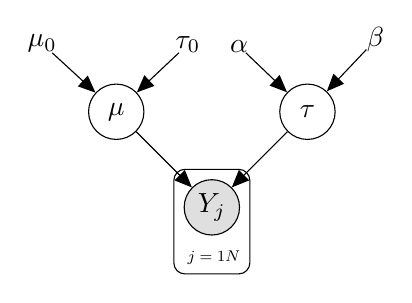
\begin{tikzpicture}
      \node[obs] (y) {$Y_j$};
      \node[latent, above left = 1 of y] (mu) {$\mu$};
      \node[latent, above right= 1 of y] (tau) {$\tau$};  
        \node[const, above left=0.7 of mu] (mx) {$\mu_0$} ; %
       \node[const, above right=0.7 of mu]  (ax) {$\tau_0$} ; %
       \node[const, above left=0.7 of tau] (atau) {$\alpha$} ; %
       \node[const, above right =0.7 of tau]  (btau) {$\beta$} ; %
	\edge{mx,ax}{mu}
	\edge{atau,btau}{tau}	
	\edge{mu,tau}{y}
	
	\plate {obs} {(y)} {\scalebox{.7}{$j=1\ld N$}} ;

	
    \end{tikzpicture}
    }
  \end{center}
  \caption{A detailed Bayesian network for the variable $Y$, which is assumed to follow a Gaussian distribution with mean $\mu$ and precision $\tau$. $Y$ is observed $N$ times.}
  \label{fig:bayesLearnDetail}
\end{figure}



\figref{bayesLearnDetail}  shows a detailed description of the model for a single variable $Y\sim N\left(\mu,\tau^{-1}\right)$. Prior information about the parameters by assuming $\mu\sim N\left(\mu_0, \tau_0^{-1}\right)$ and $\tau\sim\Gamma(\alpha,\beta)$. The dataset $\calD$ holds  $N$ \textit{i.i.d} observations of $Y$ enabling us to calculate $p(\mu,\tau\given\calD, \mu_0,\tau_0,\alpha,\beta)$. Since the prior distributions are kept inside the conjugate exponential family, the calculation is efficient both in terms of space and time complexity. 

It follows that the learning functionality in AMIDST will rest  heavily on the implementation of the core components in the toolbox (variables, distributions, Bayesian networks, etc.) as well the design to accommodate efficient (approximate) inference using these core components. The implementation of inference engines will constitute a key component for the learning implementation because  efficient and scalable \textit{inference} is both a requirement and a  guarantee for efficient and scalable \textit{parameter learning}. The next section will therefore discuss the top-level design of the AMIDST toolbox, first describing the core components, thereafter moving to the design of the inference and learning components. 









% 3. How the design of the toolbox (open-source system) is made to enable (simplify) the later implementation of learning.
%This is just the parts of the document on requirements analysis related to learning.
% !TEX root = D41-report.tex
\section{HL -- Design}\label{sec:design}

\comment{This section will cover the design of the SW, as specified through the requirements engineering document. Only the parts related to learning will be covered.}






% \documentclass[11pt]{article}

% \parskip 6pt % 1pt = 0.351 mm
% \parindent 0pt

% \usepackage{graphicx}				% Use pdf, png, jpg, or eps§ with pdflatex; use eps in DVI mode
% \usepackage[draft]{fixme}

% \newcommand{\comp}[1]{\emph{#1}}

% \begin{document}


% 1. Describe general SW-learning architecture

% 2. Link it to the design of the "core components"

% 3. Link the different components to the tasks in the WP

% 4. Link to class diagrams in the appendix
 
% 5. Summary of the parts of the design that has been implemented



\subsection{The learning module}

The core components of the modeling framework has been designed and implemented to facilitate an easy
integration with the inference and learning modules developed as part of Work packages 3 and 4. Figure~\ref{fig:design-learning} 
shows a high-level overview of the key components of the AMIDST software tool that is directly
related to learning; these learning-related components are connected to the framework core (see Section~\ref{sec:core-module}) through the \comp{Inference}
component and the \comp{PGM} component (shown using boxes with sharp corners).   

  \begin{figure}[htbp]
    \centering
    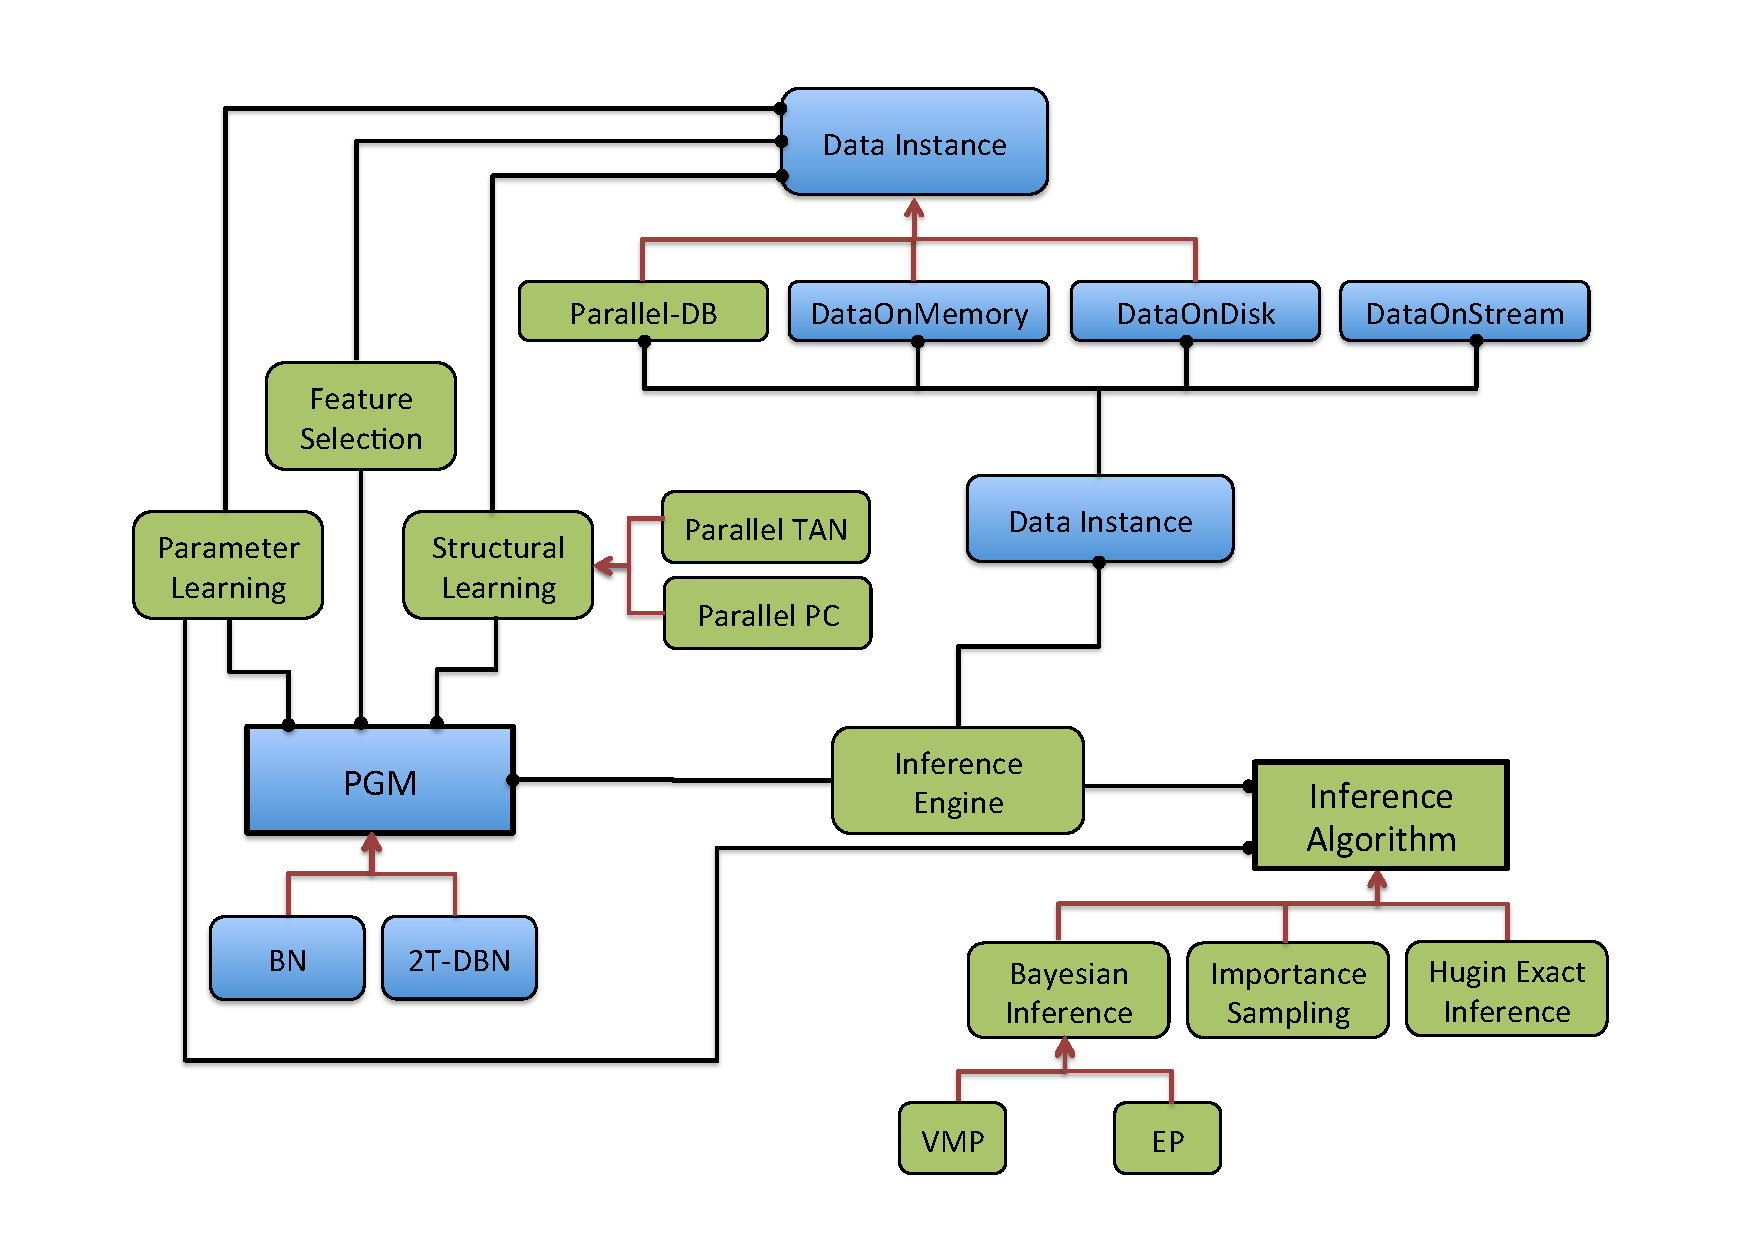
\includegraphics[width=1.05\linewidth]{design-learning2}
    \caption{Illustration of the design of the software components related to model learning. }
    \label{fig:design-learning}
  \end{figure}

In the AMIDST framework we consider two types of data sources for learning: i) Streaming data, where data arrives at high
frequency with no storage of historical data (except for data in the most recent past, which is stored in a
buffer), and 2) static databases that simply correspond to traditional databases. The database support is
realized by a general database component (\comp{Database}) that defines the database interface from which more
specialized databases (\comp{DataOnMemory}, \comp{DataOnDisk}, and \comp{ParallelDatabase}) can be derived:
\begin{itemize}
\item \comp{DataOnMemory} implements database functionality for data sets that can be loaded into main memory.
\item \comp{DataOnDisk} provides functionality for handling datasets too large to be loaded in main memory.
\item \comp{ParallelDatabase} implements a distributed database.
\end{itemize}
The employed design is intended to support future users and developers of the AMIDST toolbox in the
potential design
and implementation of other
database specifications; the only restriction being that new database components should implement the interface defined by the
\comp{Database} component. 

Functionality for handling data streams is implemented by the \comp{DataOnStream} component that allows data
to be \emph{pushed} to the AMIDST system (in contrast to a pull-approach that is standard when dealing with static
database). To allow for variation in the run-time performance of the system a buffer component
(\comp{Buffer}) is needed for storing the most recent unprocessed cases. Each of the data sources are
furthermore connected to the \comp{Data Instance} component. This component consists of a single class
that can represent a particular evidence configuration, such as the observed values of a collection of variables at
time $t$ or a particular row in a database. 

Implementations of structural learning algorithms will be realized through the \comp{Structural learning}
component and its specialized sub-classes. The design includes components for supporting PC and TAN
learning in a parallel setting (cf.\ Task 4.1). Currently, the corresponding implementation supports standard PC
learning and parallel TAN learning by interfacing to the Hugin API. 

As described in Section~\ref{sec:learningAsInference} we pursue a fully Bayesian approach for doing parameter learning in the AMIDST
framework (cf.\ the activities in Task 4.2 and Task 4.4). This, in turn, means that parameter learning reduces
to the task of inference for which  we
plan to consider two approaches: variational message passing (positioned in a variational Bayes framework and implemented in the \comp{VMP} component) and
expectation propagation (implemented in the \comp{EP} component); both components are derived from the more
general \comp{Inference} component. Particular efficient
implementations of both variational inference and expectation propagation can be realized when the distribution families of the models are
conjugate-exponential. In this case the inference operations can be further supported by specifying the
exponential distributions using their natural parameters, see Section~\ref{sec:learningAsInference}. These improvement are realized
through tailored exponential family implementations of the standard distributions that are part of the AMIDST framework
(such as the conditional linear Gaussian distribution). Note that the design of this parameter learning part of
the overall AMIDST framework is flexible in the sense that it easily accommodates potential future learning-based extensions of
the framework, e.g., Bayesian learning based on importance sampling or maximum likelihood learning using the
expectation maximization algorithm (see also
Section~\ref{sec:learningAsInference}).   

Variable selection is handled in the corresponding component in Figure~\ref{fig:design-learning}, which is
connected to both the model component (\comp{PGM}) and the \comp{Database} component. 

The high-level design description above provides an overview of the current design of the AMIDST software
framework with particular focus on the components that are directly related to model learning. The current
status of the software implementation in relation to this design is as follows:
\begin{itemize}
\item The core components (marked as blue in Figure~\ref{Figure:ToolboxBasicStructure}) has been implemented. This includes data structures
  for variables, graphs, Bayesian networks, dynamic Bayesian networks, key distributions such as multinomial
  and conditional linear Gaussian distributions represented in both standard form and as exponential families.
\item Components defining data source management functionalities have been implemented, which includes support
  for handling static database (on disk and in memory) as well as streaming data.   
\item Methods for transforming AMIDST models to and from Hugin has been implemented based on the Hugin API.  
\end{itemize}
Please see the appendix for the class diagrams for the implemented components.



\emph{Remark: The implementation is still ongoing and will continue so until the deliverable is
  submitted. Thus I expect that we will be able to expand the above list a bit. In particular, I know that
  there is currently work going on to provide parallel TAN learning in the AMIDST toolbox by calling the Hugin
  API. This would also be demonstrated at the review meeting.}  















%\end{document}

%%% Local Variables: 
%%% mode: latex
%%% TeX-master: "D41-report"
%%% End: 



% 4. Updates from Task 4.1, with focus on the actual tool-box implementation of parallel PC. We have two sources of information/ideas how to proceed: 
% a) The slideset/poster we discussed some time ago.
% AS: Also, Hugin people are investigating lines for parallelizing the PC using  multi-thread and relying on the TAN-PGM paper.
%
% b) The TAN-approach. You said you'd be able to implement this, but I'm unsure how you'll proceed. Will the postdocs supply the features you need to get this done by Christmas?
%
% AS: Anders suggested me that we could include the PGM paper (except maybe the experiments, that could be reported in D5.X)
% in D4.1. In this way there would be no rush for having it implemented in the toolbox.

% !TEX root = D41-report.tex


\section{AS -- Task 4.1: Parallelization of structural learning}\label{sec:parallel}



This section will give updates from Task 4.1, with focus on the actual tool-box implementation of parallel PC. We have two sources of information/ideas how to proceed: 
\bit
\item The slideset/poster we discussed some time ago.
\item Hugin people are investigating lines for parallelizing the PC using  multi-thread and relying on the TAN-PGM paper.
\eit

We should also discuss the learning of TAN classifiers (the PGM paper). Anders has suggested to Antonio that we could include the PGM paper here (except maybe the experiments, that could be reported in D5.1).
In this way there would be no rush for having it implemented in the toolbox.

The setup of this section is that we show in practice how the initial procedures described in the design section is to be used in practice. 

% 5.  Very preliminary thinkings from T4.2, T4.3, T4.4. 
% Perhaps there is no need to include anything specific from these tasks, beyond what is concerned with the requirement analysis.
 
%% !TEX root = D41-report.tex
\section{HL -- Initial results from the other tasks} \label{sec:otherTasks}

\comment{This section will discuss any results or ideas that have been developed in Tasks 4.2, 4.3, 4.4. 
Not much to include. Maybe delete?}


\section{Conclusion}

This document summarizes the progress of the software development related to learning functionality in the AMIDST toolbox. Parameter learning functionality rests heavily upon efficient design and implementation of core components and inference engines, and these parts were therefore discussed in some detail. Structural learning is ongoing (in Task 4.1) and will be finalized in Month 15. A preliminary discussion of the results was given.
Implementation of dedicated functionality for parameter learning (Em algorithm and similar) has not yet started, and is not discussed.

\addcontentsline{toc}{section}{\numberline{}\textbf{References}}

\bibliographystyle{splncs}
\bibliography{biblio}



\end{document}  